\chapter{Systematic uncertainties}\label{chap:systematics}
\section{Trigger efficiency}
Systematics on the trigger efficiency changes with the multiplicity. Given that the efficiency was determined \cite{pPb_mbsptrk_trigger} using a detector under different conditions and for a different collision system, we assign to the efficiency $\epsilon_{\mathrm{trigger, pp}}$ for (loosePrimary + d0) track multiplicity == 2 absolute systematic uncertainty of 0.5 \%, for (loosePrimary + d0) track multiplicity > 2 \&\& < 5 an absolute systematic uncertainty of 0.1 \% and for multiplicity > 5 no systematic uncertainty. In the case of less than 2 tracks, no correction for the trigger efficiency was applied as these cases contribute negligibly to the $\RAA$.

\section{Vertex reconstruction efficiency}
Removing the beam background was not applied to determine the vertex reconstruction efficiency, which would likely lead to a sub-\% systematic effect based on \cite{chargedHadroninPP2010}. Major systematic errors probably arise from the assumption that the vertex reconstruction efficiency can be taken independently in events with multiple vertices. For this reason, we assign a rather safe 1\% absolute systematic till Pythia studies can be run. 

\section{Vertex merging correction factor}
The toy Monte-Carlo model described in Section~\ref{sec:vertex_merging} has several input parameters which generate systematic uncertainty on $\varepsilon_\text{m}$. The sources of systematics are the following:
\begin{enumerate}
    \item Poisson distribution parameter $\lambda$ of truth-level distribution of $\nvtx$, which taken from data and tuned iteratively. The model shows that for a chosen value of $\lambda$, the mean of the observed distribution drops by approximately 0.2 (compared to the truth). This value varies around the initial parameter. The model is rerun with $\lambda\pm0.2$ and the maximum of relative (to central value) deviation is plotted. The error is estimated from a constant function fit to the relative deviations distribution (see Figure~\ref{fig:sys_eps_m_nvtx}) and quoted as $0.4\%$.
    \begin{figure}[h]
        \centering
        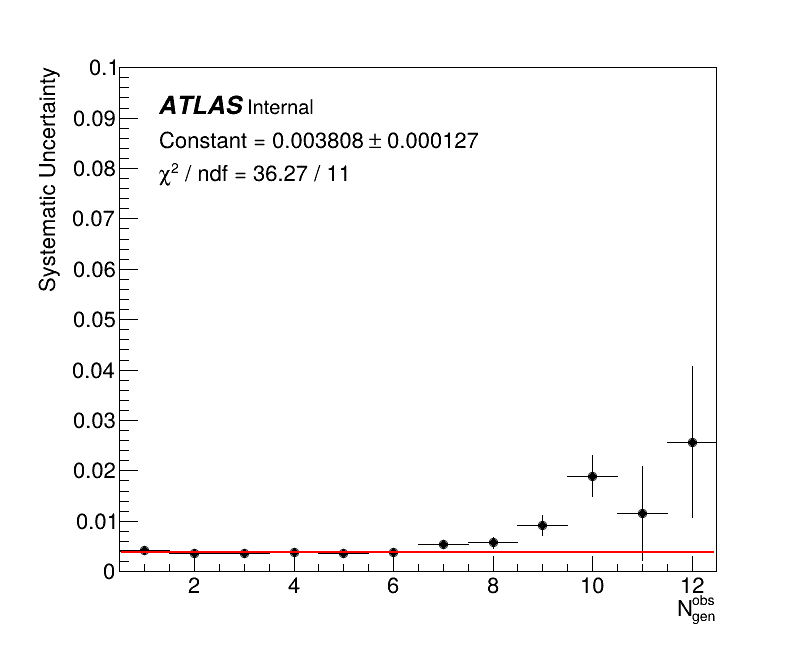
\includegraphics[width=0.5\linewidth]{images/sys_unc_mean_vtx.png}
        \caption{Systematic Uncertainty of $\varepsilon_\text{m}$ for variations of $\lambda$}
        \label{fig:sys_eps_m_nvtx}
    \end{figure}
    \item The relative normalization of functions $f_1$ and $f_2$ (Section~\ref{sec:vertex_merging}), which is extracted from the fit to real data. Choice of the normalization drives the merging probability for very small $\Delta z$. To estimate the effect of the normalization parametrization, the $A_1$ parameter of $f_1$ extracted from the fit is varied up and down according to its uncertainty. The result is shown on the left of Figure~\ref{fig:sys_eps_m_bw_amp}. The parameter $\Gamma$ defines the "effective" merging region for vertices and varies within its uncertainty (the right side of Figure~\ref{fig:sys_eps_m_bw_amp}). Resulting uncertainties are $0.1\%$ and $0.05\%$.
    \begin{figure}[h]
        \centering
        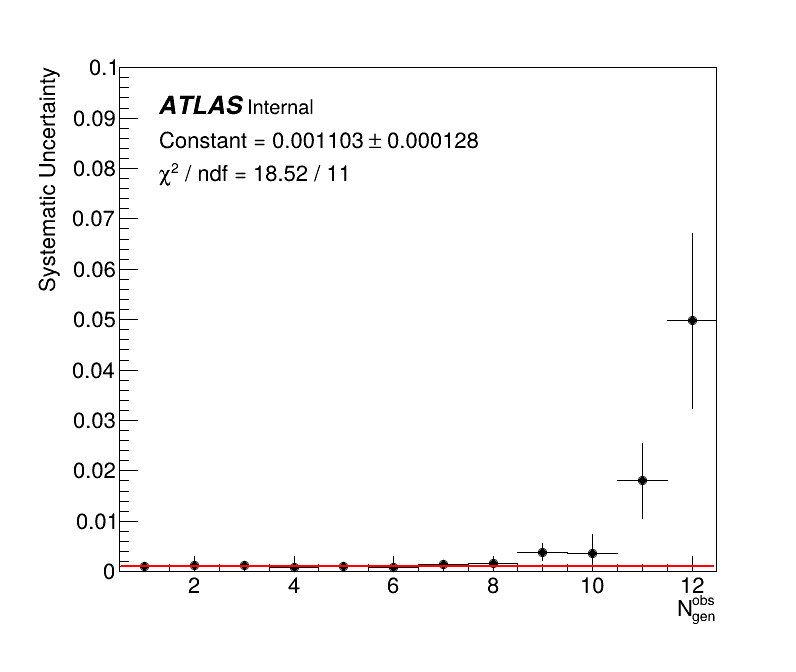
\includegraphics[width=0.48\linewidth]{images/sys_unc_dg_amplitude1.png}
        \hskip10pt
        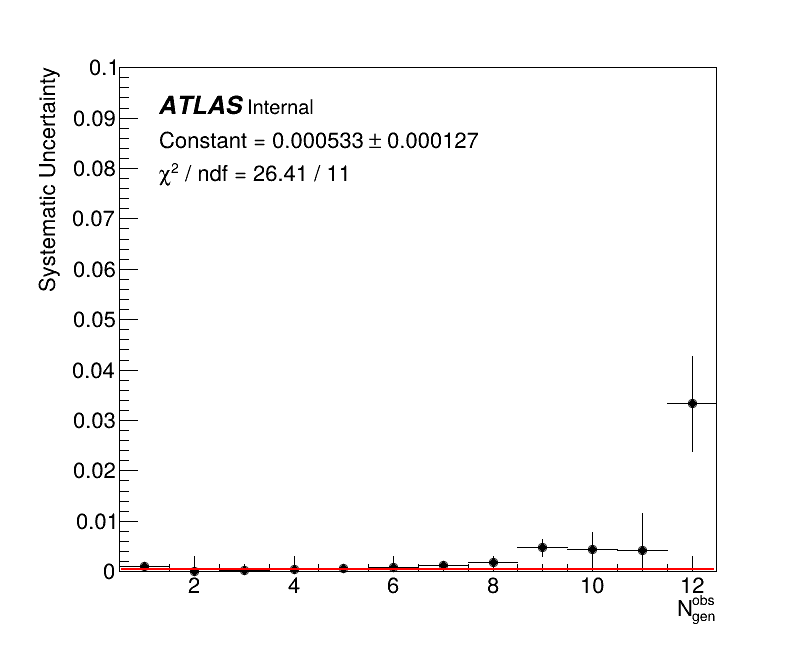
\includegraphics[width=0.48\linewidth]{images/sys_unc_dg_sigma1.png}
        \caption{Systematic Uncertainty of $\varepsilon_\text{m}$ for variations of $A_1$ (left) and $\Gamma$ (right)}
        \label{fig:sys_eps_m_bw_amp}
    \end{figure}
    \item The width of the $\zvtx$ distribution for a single vertex. The generated distribution is about $1.3\%$ wider after merging. The effect of varying the input width of $\zvtx$ by this amount results in $0.1\%$ systematic (Figure~\ref{fig:sys_eps_m_zvtx}).
    \begin{figure}[h]
        \centering
        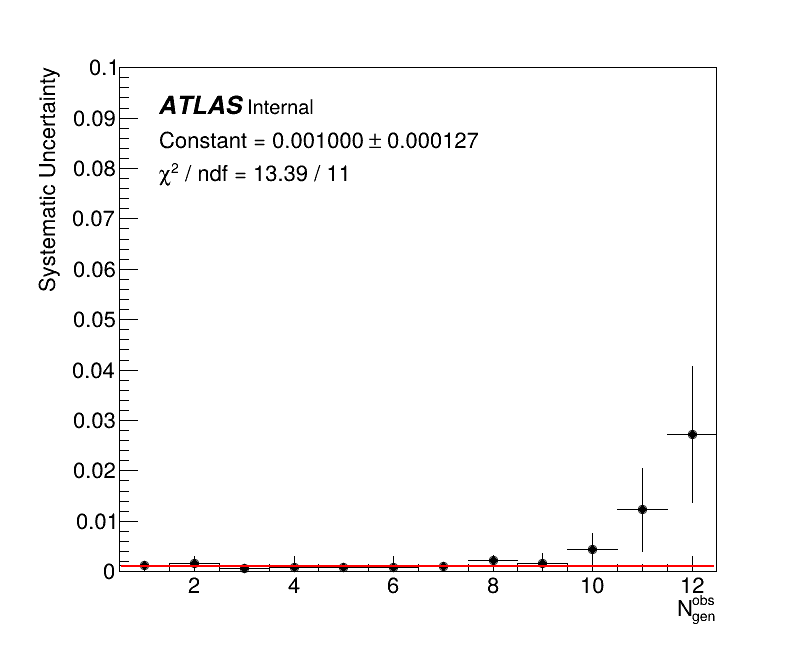
\includegraphics[width=0.5\linewidth]{images/sys_unc_z_vtx_sigma.png}
        \caption{Systematic Uncertainty of $\varepsilon_\text{m}$ for variations of width of $\zvtx$}
        \label{fig:sys_eps_m_zvtx}
    \end{figure}
    \item The algorithm used for merging vertices. Two of the proposed algorithms were compared and are consistent throughout the whole $N_\text{gen}^\text{obs}$ range, no systematic effect is visible. No systematic uncertainty is assigned due to this choice.
\end{enumerate}
The total systematic uncertainty is calculated as the quadratic sum of these sources and equals $0.4\%$. % 0.43 to be precise
\section{Glauber modeling -- $\avgNcoll$}
Calculation of $\avgNcoll$ within the Glauber model is associated with the following systematic uncertainties:
\begin{enumerate}
    \item Underlying geometric model of nuclei. Two models for $\OO$ were used, 3pF and Wave-function (Section~\ref{sec:ncoll_glauber}). While keeping all other parameters fixed, the change in the model choice yields a difference of $3.5\%$ in the resulting $\avgNcoll$.
    \item Uncertainty of parameters of 3pF. Each parameter was varied within its known uncertainties from \cite{DEVRIES1987495}
    \item Uncertainty of inelastic cross section $\sigma_{NN}$. It was varied up and down within $\pm\qty{0.6}{mb}$ (Section~\ref{sec:ncoll_glauber})
    \item Minimal distance between nucleons $d_\text{min}$. If a given nucleon is sampled "too close" to another nucleon, its position is resampled, which introduces bias in the generated geometry. Uncertainty due to choice of this parameter is calculated by varying $d_\text{min}$ from 0.0 to 0.8 fm \cite{PhysRevC.97.054910}
    % \item Nucleon profile parameter $\omega$. It was varied up and down by $0.1$ to propagate uncertainty to $\avgNcoll$
\end{enumerate}
Each parameter was varied around its central value, and the average of absolute deviations is quoted as systematic uncertainty for a given source (Figure~\ref{fig:systematics_ncoll_oo_nene})
\begin{figure}[h]
    \centering
    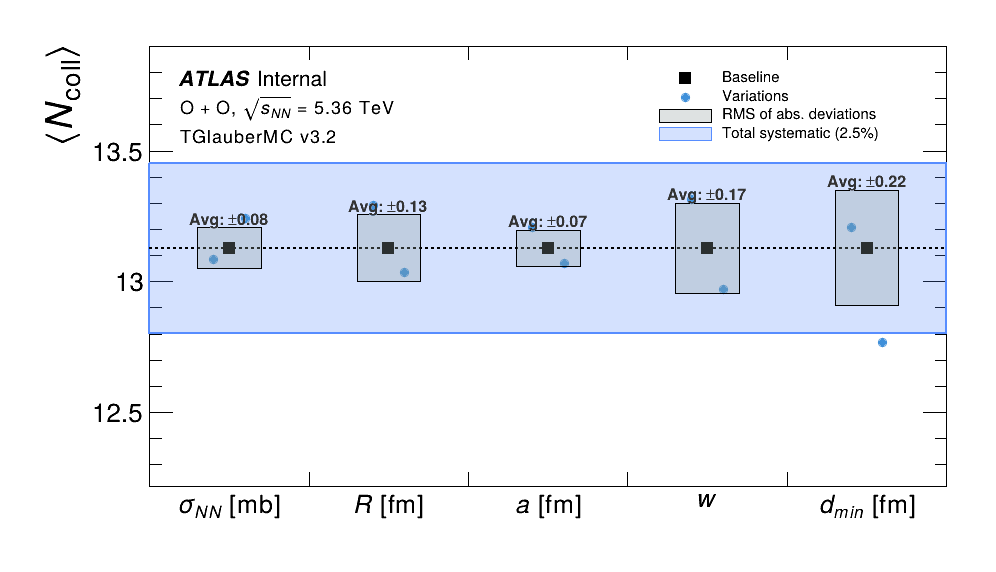
\includegraphics[width=0.8\linewidth]{images/ncoll_sensitivity_OO.png}
    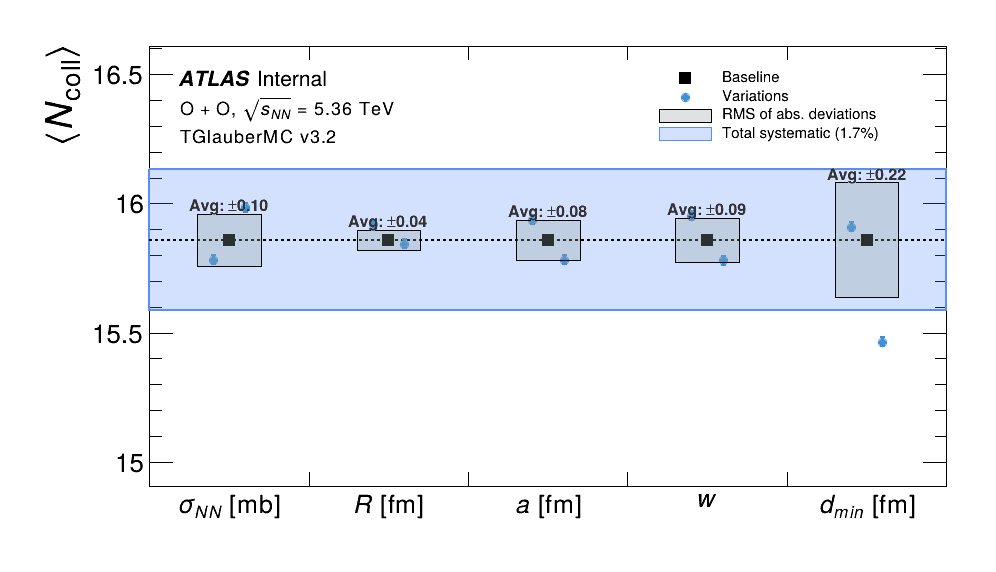
\includegraphics[width=0.8\linewidth]{images/ncoll_sensitivity_NeNe.png}
    \caption{Top: summary of systematic uncertainties for $\OO$ (except geometry model). Bottom: summary for $\NeNe$}
    \label{fig:systematics_ncoll_oo_nene}
\end{figure}
After summing up the geometry choice and the parameter variation systematics, the uncertainty on $\avgNcoll$ reaches $4.3\%$ for O.

\section{Contamination of $\Oa$ and $\alal$}
There are three sources of systematic on correction for the $\OO$ contamination by $\Oa$ and $\alal$ collisions:
\begin{enumerate}
    \item The model dependence of $\Npart$ or $\tpv$, where the Glauber, Hijing, and Angantyr models were studied along with modifications originating in previously published measurements. The difference in their scaling, observed in Fig~\ref{fig:corr_norm}, is also a source of uncertainty. 
    \item Other uncertainty is associated with the fact that collisions will run for a certain amount of time, i.e., the transmutation will start, before the data-taking status is declared at the ATLAS detector.
\end{enumerate}


%As the left part of the fig \ref{fig:ntrk_ncoll_norm} shows, the systematic on $\avgNcoll$ grows almost linearly with the uncertainty on $\langle \tpv \rangle$, which then needs to be determined. 


% Tracks used to calculate $\tpv$ are selected with a set of cuts, which assume track-to-vertex association. To eliminate dependence on cuts, one can define similar quantities (which are just averages over a given event record)
% \begin{equation}
%     \avgtpvreco = \frac{N_\text{trk}^\text{reco}}{N_\text{vtx}}, \quad 
%     \avgtpvsel = \frac{N_\text{trk}^\text{sel}}{N_\text{vtx}}, \quad 
% \end{equation}
% for any given event and compare them {\red (stability of $\avgtpvreco$ is also ''known'', its flat within $2\sigma$)}. Given that these quantities do not depend on $\mu$ in the limit of small $\mu$ ($\sim 0.2$, see sec.~\ref{sec:transmutation_correction}), they should also be constant (in time) in the absence of contamination, which is the case for $\pp$ collisions. To quantify the systematic uncertainty related to choosing some cuts over not using them at all, the ratio $\avgtpvsel/\avgtpvreco$ is constructed. Its RMS around the mean value across the available $\pprefSample$ low-$\mu$ sample is quoted as the systematic uncertainty of $0.2\%$ (see fig.~\ref{fig:tpv_sys_lowmu_highmu}).
% \begin{figure}[h]
%     \centering
%     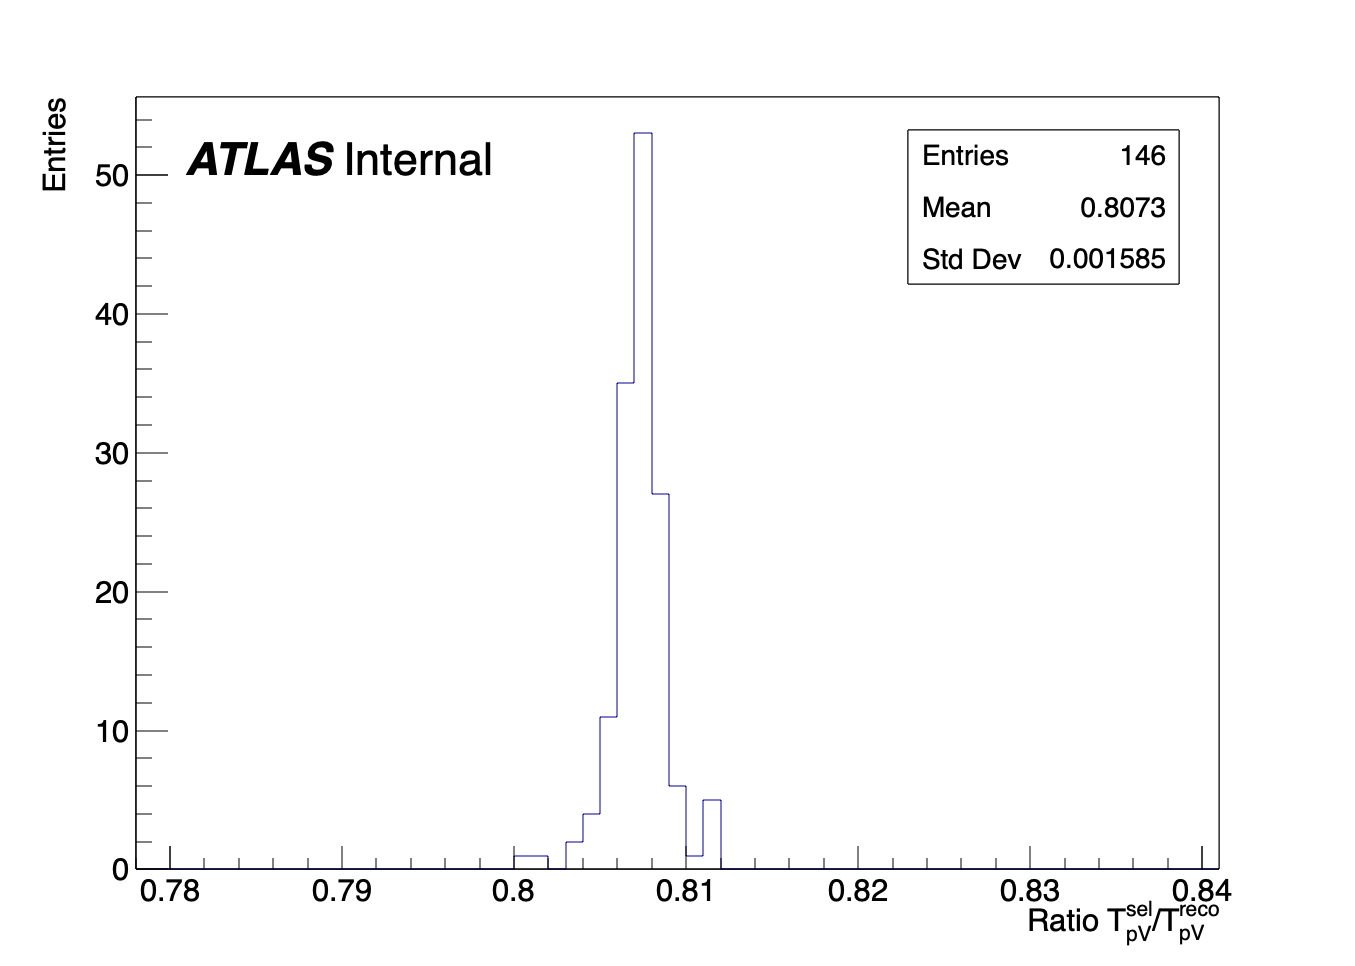
\includegraphics[width=0.45\linewidth]{images/tpvsel_tpvreco_lowmu.png}
%     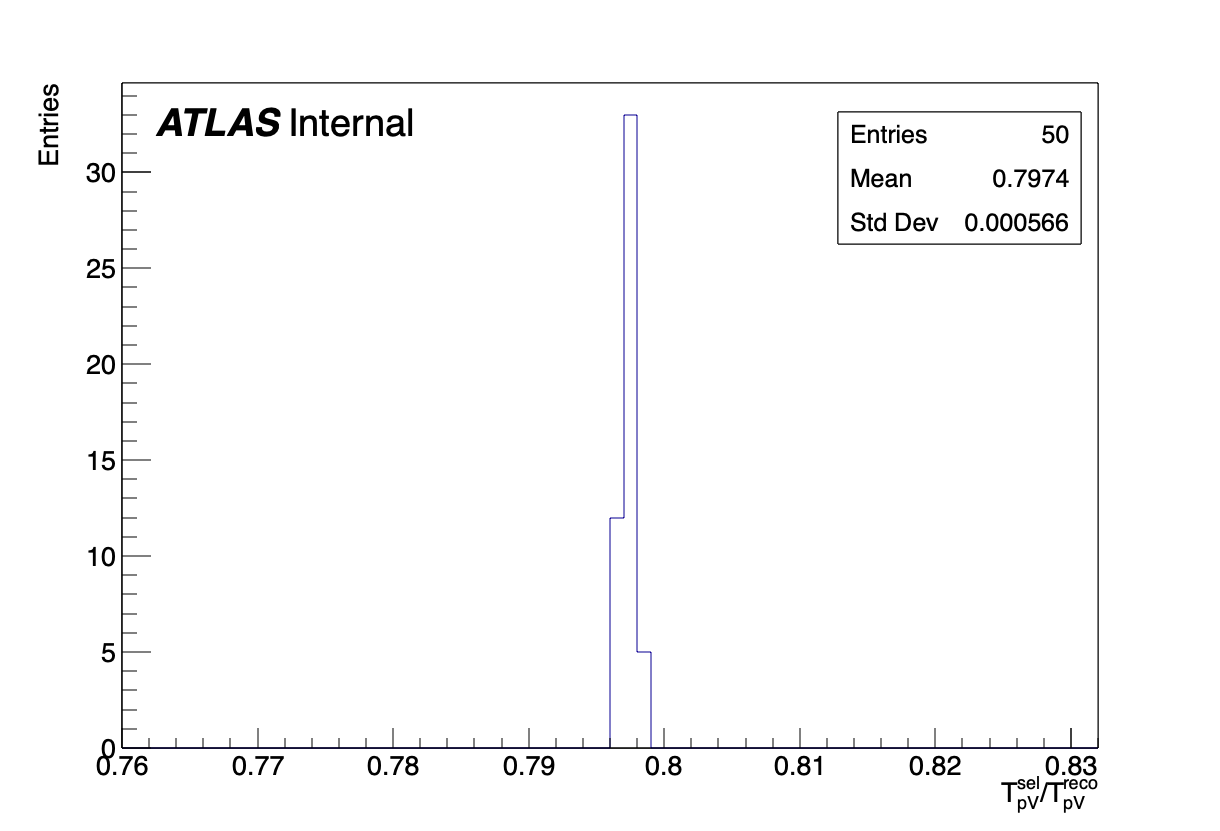
\includegraphics[width=0.45\linewidth]{images/tpvsel_tpvreco_highmu.png}
%     \caption{Ratios of $\avgtpvsel/\avgtpvreco$ for LB where $\mu\sim\text{const}$. Left: $\langle \mu\rangle\sim 0.2$. Right: $\langle \mu \rangle \sim 4.0$}
%     \label{fig:tpv_sys_lowmu_highmu}
% \end{figure}

%The ratio of $\tpv(t_1)$ at any given time to $\tpv(0)$ (representing start of the run where no contamination is present) should be equivalent to same ratio from MC (e.g. HIJING), as all the efficiencies and corrections cancel, if we assume conditions to be constant throughout the run. The same argument applies to $\avgtpv$. Therefore, to quantify conservatively the effect of choosing cuts for $\tpv,$ one can plot the above-mentioneded ratios as a function of time (lumiblock) and compare them ({\red e.g., fit absolute deviations with a constant function and quote it as systematic})

\section{Difference in conditions}
{\blue Will be determined from a comparison of full-sim Pythia MCs with different conditions}
\section{Gap cut} 
{\blue Will be determined when MC Pythia samples for various diffraction modes are available, based on variations of the cut value and the mismatch of the inclusive MC on the data $\forwardgap$ distributions.}


